\section{Theory}\label{Theory}

\subsection{Gyrotron guns}
\begin{itemize}
\item{A few words on gyrotrons}
\item{What they are used for}
\item{GT-170: image}
\item{Possible disruptions in the use of gyrotrons}
\item{Has this been quantified ? Time scale ? Densities ? Clouds}
\end{itemize}

\subsection{The FENNECS code}
\begin{itemize}
\item{Particle In Cell code}
\item{Brief description of implementation}
\item{Vlasov Poisson system of equations}
\end{itemize}

\subsection{Ion-Induced Electron-Emissions}
\begin{itemize}
\item{Schou's model}
\item{Kinetic emissions}
\item{Low energies: potential emissions}
\item{Possible cascade phenomena}
\end{itemize}


In order to take into account IIEE in the FENNECS code, the question of choosing the appropriate physical model arose. Indeed, expected energy distribution of the ions in the TREX experiment was ranging between 0 and 20-30 keV. These values correspond to roughly the minimal and maximal values that could be reached by ions accelerated in an electric field perpendicular to the magnetic field lines, in vacuum, and over a distance of about 1cm.
 
\begin{figure}[h!]
\centering
	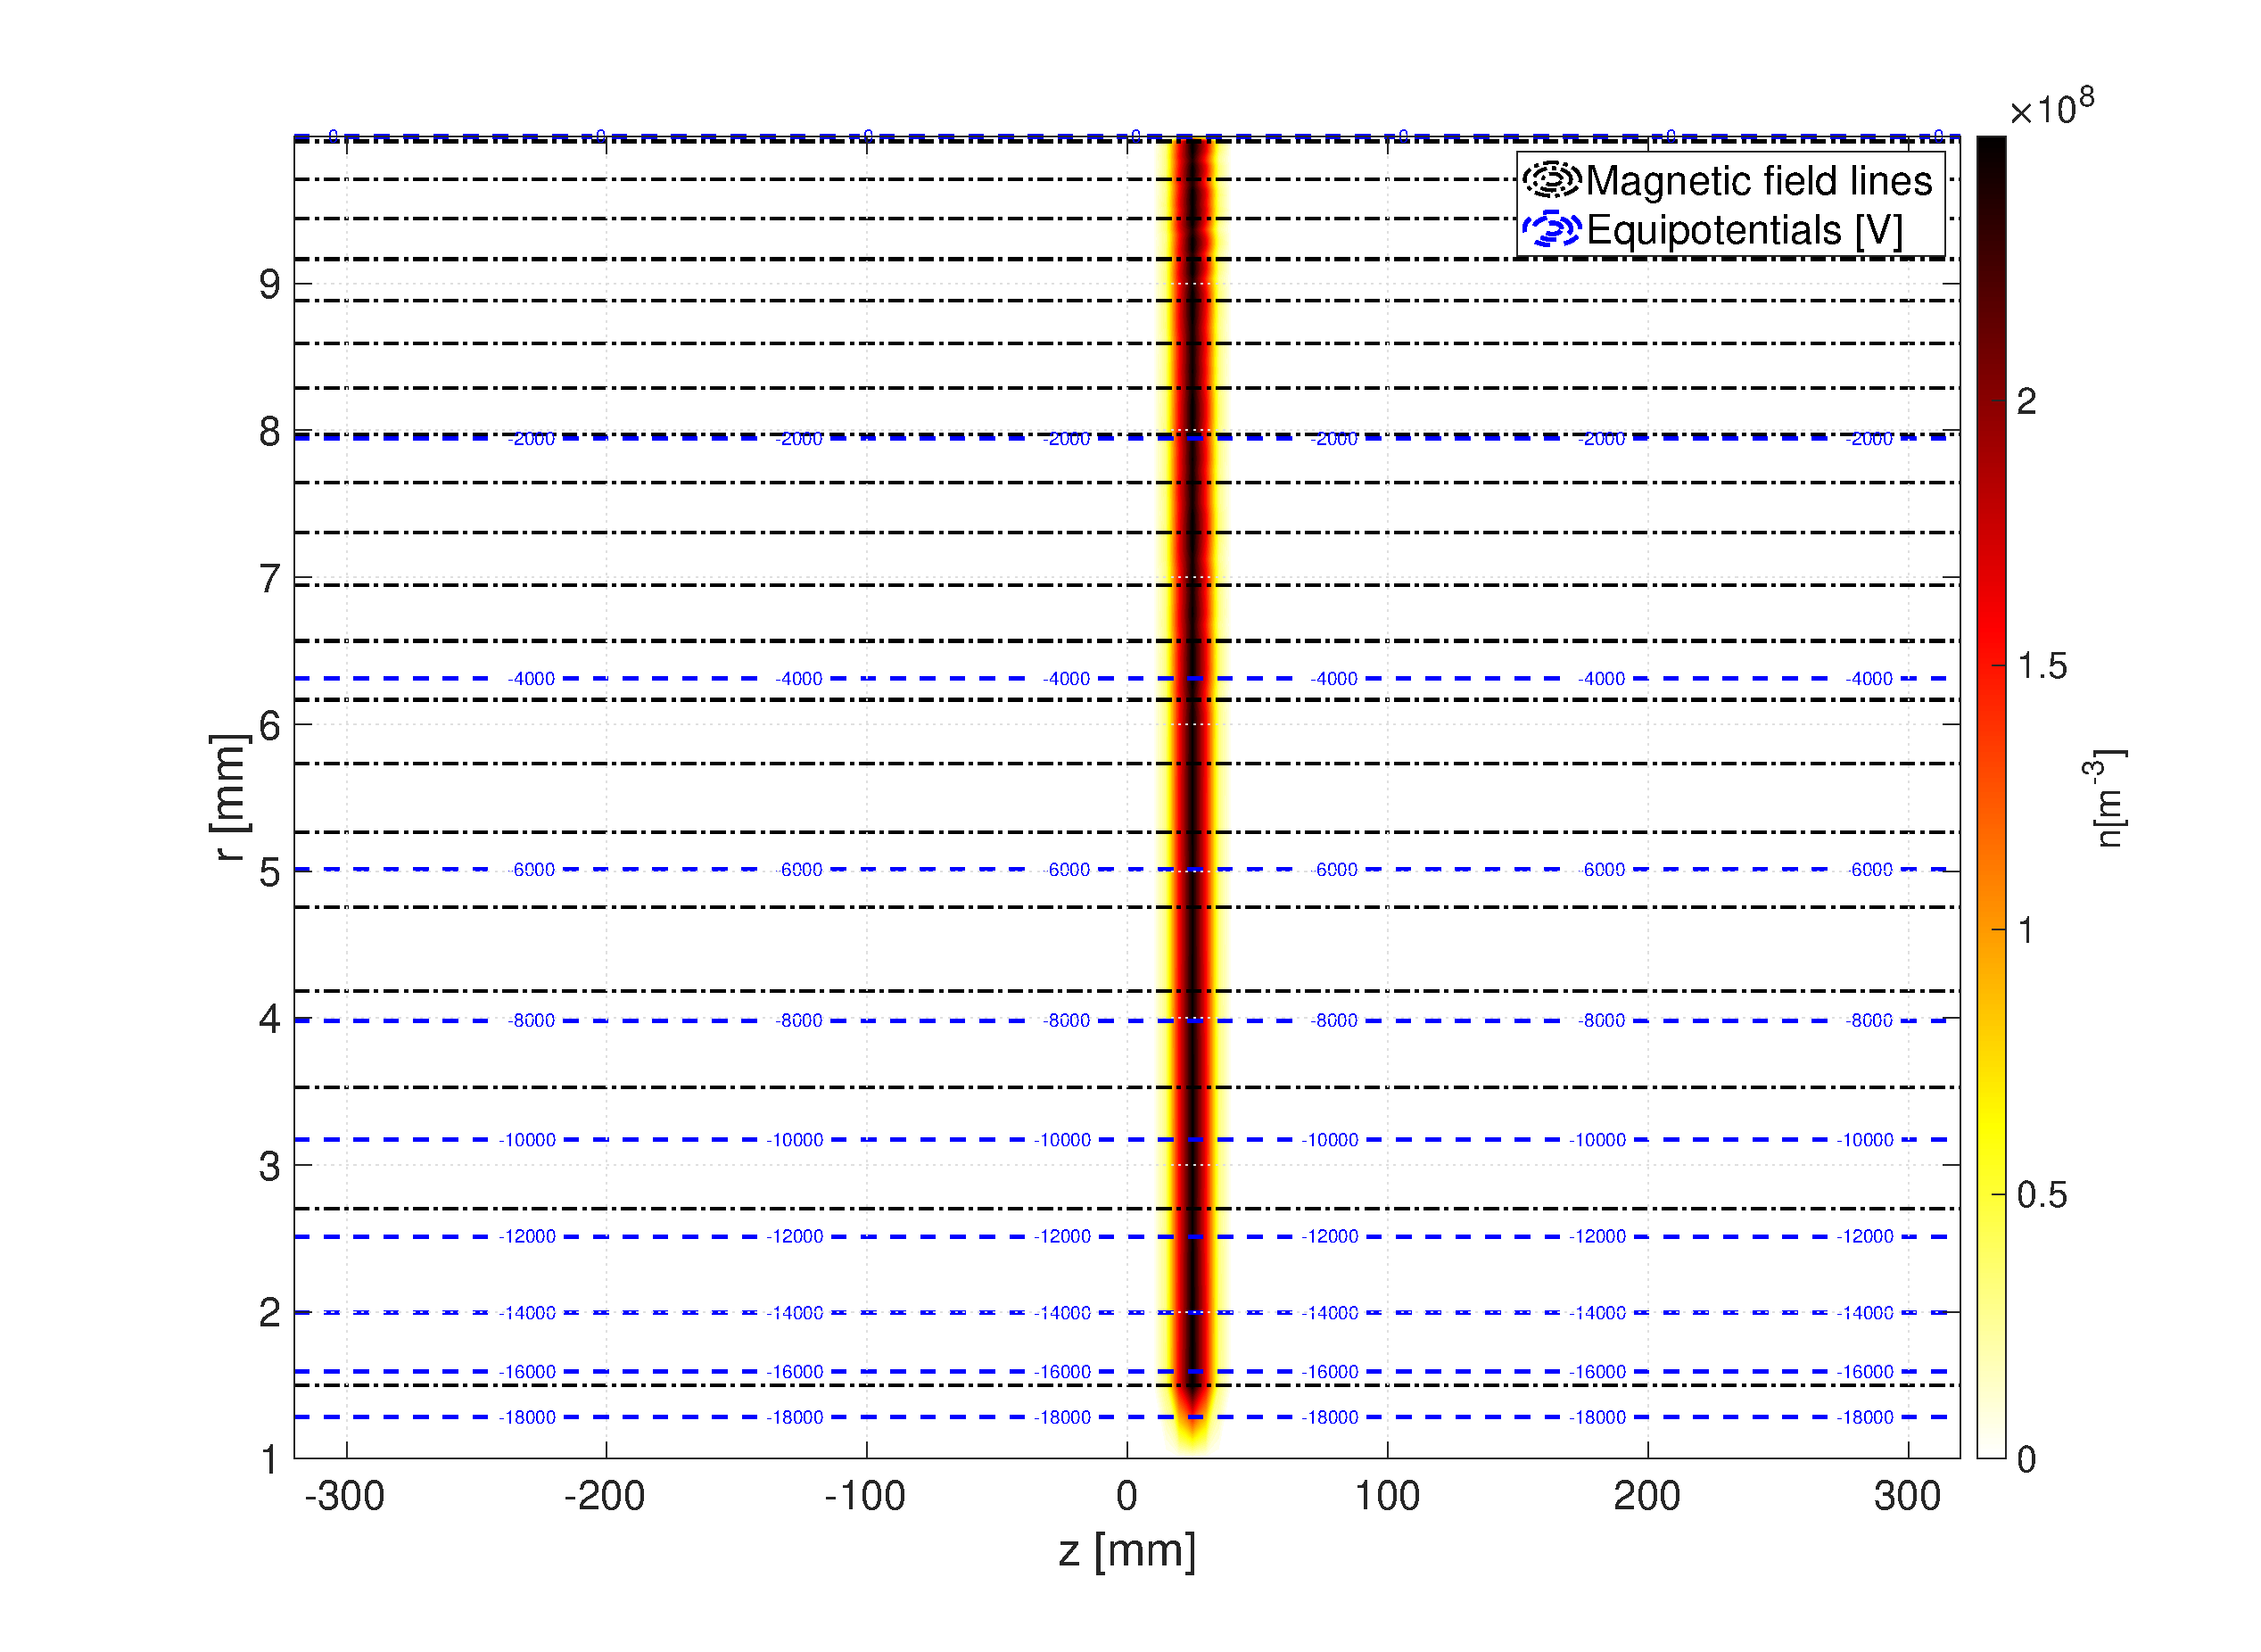
\includegraphics[width = 0.75 \textwidth]{Configuration_ions.eps}
	\caption{\label{Config_ions} Initial ion configuration in ($R,Z$) plane. The geometry is coaxial.}
\end{figure}  

\noindent Fig.(\ref{Config_ions}) shows the initial distribution of protons in the coaxial geometry where the electric equipotentials are plotted in blue, and the magnetic field lines in black. In this particular configuration, in vacuum, the acquired energy of the protons when they reach the cathode follows 

\beq
E(r_0) = \Delta \Phi \frac{\log{(\frac{r_0}{r_a})}}{\log{(\frac{r_b}{r_a})}},
\eeq

\noindent where $r_0$ is the initial proton radial position, $\Delta \Phi$ the potential bias between the cathode located at $r_a$ and the anode located at $r_b$. Thus, taking numerical values such as $\Delta \Phi = 20$kV and evaluating $E(r_a)$ and $E(r_b)$, one get that $E\in [0,20]$ keV. This way, a model describing IIEE in this energy range had to be found. 

\noindent Regarding the model in itself, one had to consider that IIEE would be dependent on the material constituting the electrodes. Indeed, protons impinging on stainless steel would not have the same effect as if they were striking a copper electrode. The electron yield would also depend on the energy of the incident particle. It was expected that the number of released electrons would be different if the ion hit the cathode at high or low energy. At this point, nothing ensured that the type of interaction between ion an electrode would be the same on the whole energy range. It was also expected that the electron yield would depend on ions parameters: mass $m$, charge $q$ or charge to mass ratio $q/m$ for example.\\

\noindent With these considerations, one model drew our attention: Schou's model, derived by Schou in 1980. Our motivation for a qualitative (at first) survey of these ion-induced electrons drove us towards this model in particular, since it distinguishes itself by its remarkable simplicity. Following the description of Schou's model from \cite{HasselII}, this approach of IIEE is based on the ionisation cascade theory, and a system of Boltzmann transport equations.  Neglecting recoil ionisation in the material, the electron yield $\gamma$ takes the following form: 

\beq
\gamma = \Lambda \cdot D_e,
\eeq

\noindent where $D_e$ is the amount of energy deposited by inelastic collision at the surface, and $\Lambda$ contains cross sections dependent parameters for the interaction at a given energy and has the following form 

\beq
\Lambda = \int_0^{\infty} \frac{\Gamma_m E}{4 |dE_i/dx|(E+W)^2}dE.
\eeq

\noindent In the above expression for $\Lambda$, $E=E_i-W$, $\Gamma_m$ is a function that depends on the exponents of used power cross-sections. The term $dE_i/dx$ corresponds to the energy loss of low-energy electrons in the material. The interesting point of this model is that it is made of two independent terms, one containing target material parameters ($\Lambda$) and the other containing the impacting particle characteristics ($D_e$). Another advantage of this separated description is that it can be reformulated such that it is express in terms of the energy loss of the incident particles inside the material, which is a quantity that can be measured easily, and for which tabulated numerical values exist. Thus, denoting by $dE/dx\Big|_i$ the energy loss of ions in the electrode material, one can write the electron yield as follows: 

\beq
\gamma = \Lambda \cdot \beta \cdot  \frac{dE}{dx}\Bigg|_i.\label{Schou}
\eeq

\noindent In Eq.(\ref{Schou}), $\beta$ accounts for energy transport by recoiling electrons and backscattered ions. One point that it is important to be emphasized, is that Schou's model is a kinetic model that holds for substantially high energies, that is above 1keV. For energies below, Schou's theory has to be replaced by another model, in which kinetic emissions are replaced by the so-called potential emissions.\\

The potential emissions model that has been chosen to treat ion-induced electron emissions at low energies ($E<1$keV) is due to Kishinevsky \cite{Kishi73}. The result is very elegant in the sense that it depends only on the Fermi energy of the material, the ionisation energy required to produce the incident ions, and the work function of the metal. Since no energy dependence of the electronic yield arises in this model, the yield should be constant in the range $[0,1]$ keV. Comments on the validity of this approximation will be made below. Let us now briefly summarise the derivation of the result for $\gamma$. First, let us state the expression for the electronic yield as derived in \cite{Kishi73}: 

\beq
\gamma \sim \frac{0.2}{\epsilon_F}\big( 0.8 \cdot E_i -2 \phi \big),
\eeq

\noindent where $\epsilon_F$ denotes the Fermi energy of the metal constituting the target material, $\phi$ its work function, and $E_i$ the ionisation energy required initially to produce the incident ions. For hydrogen, this ionisation energy is $E_H \simeq 13.6$ eV. 

\subsection{Trapped Electrons EXperiment TREX}
\begin{itemize}
\item{Description of the experiment}
\item{What we hope to see}
\item{Comparisons with our module ?}
\end{itemize}

\subsection{Numerical implementation}
\begin{itemize}
\item{Find tabulated values of energy loss (material dependent)}
\item{Find tabulated values for electronic yield}
\item{Fit these values with energy polynomials of various degrees}
\item{Poisson distribution - random numbers with $\lambda=\gamma(E)$}
\item{Invert Buneman algorithm}
\item{Generate electrons at last position of lost ion with \# of electrons following Poisson}
\end{itemize}



In order to implement numerically Schou's model from Eq.(\ref{}), it was necessary to obtain reference values for the electronic yield, as a function of incident ions' energies. Tabulated values for the energy loss $dE/dx$ of protons in various materials were extracted from \cite{Janni_vol1, Janni_vol2}. To be consistent with the TREX experiment plans (See \ref{TREX_sec}), attention was drawn on 304 stainless steel $^{304}SS$, copper $Cu$ and aluminum $Al$. 
